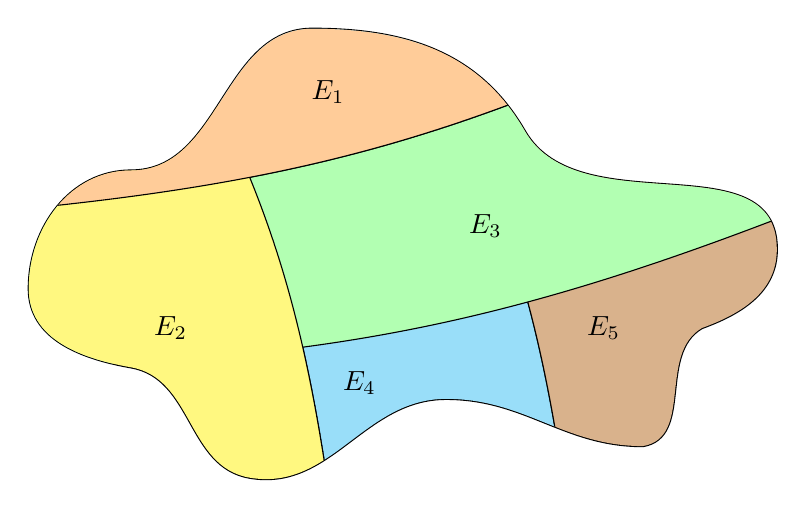
\begin{tikzpicture}
\path
  coordinate (aux0) at (0,1.5)
  coordinate (aux1) at (0,3.5)
  coordinate (aux2) at (10,3.5)
  coordinate (aux3) at (9,6)
  coordinate (aux4) at (4,0)
  coordinate (aux5) at (7,0)
  coordinate (aux6) at (2,6)
  coordinate (aux7) at (5,6)
  coordinate (esp1) at (0.2,2.5)
  coordinate (esp2) at (1.5,1.5)
  coordinate (esp3) at (3,0.1)
  coordinate (esp4) at (5.5,1.1)
  coordinate (esp5) at (8,0.5)
  coordinate (esp6) at (8.75,2)
  coordinate (esp7) at (9.7,3)
  coordinate (esp8) at (6.5,4.5)
  coordinate (esp9) at (3.8,5.8)
  coordinate (esp10) at (1.5,4)
  ;
\draw[line width=0.8pt]
  (esp1) to[out=-90,in=170]
  (esp2) to[out=-10,in=170]
  (esp3) to[out=-10,in=180]
  (esp4) to[out=0,in=180]
  (esp5) to[out=10,in=-150]
  (esp6) to[out=20,in=-90]
  (esp7) to[out=90,in=-60]
  (esp8) to[out=120,in=0]
  (esp9) to[out=180,in=0]
  (esp10) to[out=180,in=90]
  cycle;    
\clip
  (esp1) to[out=-90,in=170]
  (esp2) to[out=-10,in=170]
  (esp3) to[out=-10,in=180]
  (esp4) to[out=0,in=180]
  (esp5) to[out=10,in=-150]
  (esp6) to[out=20,in=-90]
  (esp7) to[out=90,in=-60]
  (esp8) to[out=120,in=0]
  (esp9) to[out=180,in=0]
  (esp10) to[out=180,in=90]
  cycle;    
\filldraw[fill=cyan!40]
  (aux4) to[bend right=10]
  (aux6) --
  (aux7) to[bend left=10]
  (aux5) -- cycle;
\filldraw[fill=brown!60]
  (aux5) to[bend right=10]
  (aux7) --
  (10,6) --
  (10,0) -- cycle;
\filldraw[fill=green!30]
  (aux0) -- 
  (aux1) to[bend right=10]
  (aux3) --
  (10,6) -- 
  (aux2) to[bend left=10] cycle;
\filldraw[fill=yellow!50]
  (0,0) -- 
  (aux4) to[bend right=10]
  (aux6) --
  (0,6) -- 
  (0,0) -- cycle;
\filldraw[fill=orange!40]
  (0,6) -- 
  (aux1) to[bend right=10]
  (aux3) --
  (0,6) -- cycle;
\node at (4,5) {$E_1$};  
\node at (2,2) {$E_2$};  
\node at (6,3.3) {$E_3$};  
\node at (4.4,1.3) {$E_4$};  
\node at (7.5,2) {$E_5$};  
\end{tikzpicture}